% !TeX root = ../main.tex

\documentclass[../main.tex]{subfiles}
\begin{document}

\section{Cơ sở lý thuyết về tháp giải nhiệt}
\label{sec:cooling_tower_theory}

\subsection{Nguyên lý truyền nhiệt và truyền khối}
\label{sec:heat_mass_transfer_principle}

Hoạt động của tháp giải nhiệt dựa trên nguyên lý kết hợp giữa truyền nhiệt và truyền khối, trong đó quá trình làm mát nước được thực hiện thông qua hai cơ chế chính: truyền nhiệt hiện và truyền nhiệt ẩn \cite{ashrae2020cooling}.

\textbf{Truyền nhiệt hiện} xảy ra do sự chênh lệch nhiệt độ giữa nước nóng và không khí lạnh. Khi nước có nhiệt độ cao hơn không khí tiếp xúc trực tiếp, nhiệt lượng được truyền từ nước sang không khí theo định luật Fourier về dẫn nhiệt. Quá trình này tuân theo phương trình:

\begin{equation}
    Q_{\text{hiện}} = h_c \cdot A \cdot (T_{\text{nước}} - T_{\text{không khí}})
\end{equation}
Trong đó:
\begin{itemize}
    \item $h_c$: hệ số truyền nhiệt đối lưu ($W/m^2\cdot K$)
    \item $A$: diện tích tiếp xúc ($m^2$)
    \item $\left(T_{\text{nước}} - T_{\text{không khí}}\right)$: chênh lệch nhiệt độ ($K$ hoặc $^\circ\mathrm{C}$)
\end{itemize}

\textbf{Truyền nhiệt ẩn} là cơ chế quan trọng hơn, xảy ra khi một phần nước bay hơi vào không khí. Quá trình bay hơi đòi hỏi năng lượng (nhiệt ẩn hóa hơi), năng lượng này được lấy từ khối nước còn lại, làm giảm nhiệt độ của nó. Truyền khối nước từ pha lỏng sang pha khí được mô tả bởi:

\begin{equation}
    \dot{m}_{\text{bay hơi}} = h_m \cdot A \cdot (W_{\text{bão hòa}} - W_{\text{không khí}})
\end{equation}
Trong đó:
\begin{itemize}
    \item $h_m$: hệ số truyền khối ($\mathrm{kg}/(\mathrm{m}^2 \cdot \mathrm{s})$)
    \item $W_{\text{bão hòa}}$: độ ẩm tuyệt đối của không khí bão hòa tại nhiệt độ nước ($\mathrm{kg}_{\text{hơi}}/\mathrm{kg}_{\text{không~khí}}$)
    \item $W_{\text{không khí}}$: độ ẩm tuyệt đối của không khí xung quanh ($\mathrm{kg}_{\text{hơi}}/\mathrm{kg}_{\text{không~khí}}$)
\end{itemize}

% \begin{figure}[H]
%     \centering
%     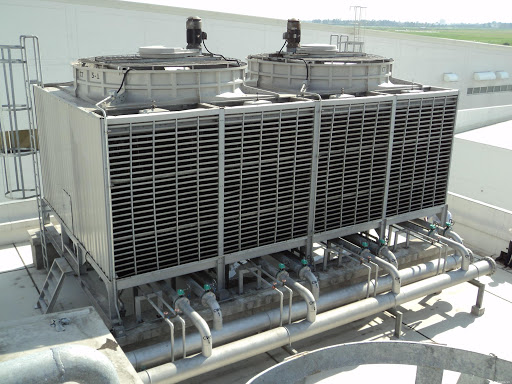
\includegraphics[width=1\textwidth]{../Hinhve/cooling_tower.jpg}
%     \caption{Tháp giải nhiệt trong công nghiệp minh họa quá trình truyền nhiệt và truyền khối}
%     \label{fig:cooling_tower}
% \end{figure}

Sự kết hợp của hai cơ chế này tạo nên hiệu quả làm mát vượt trội của tháp giải nhiệt. Khác với các hệ thống trao đổi nhiệt thông thường chỉ dựa vào truyền nhiệt hiện, tháp giải nhiệt có thể đạt được nhiệt độ nước ra thấp hơn nhiệt độ không khí xung quanh nhờ vào quá trình bay hơi. Giới hạn lý thuyết thấp nhất mà nhiệt độ nước có thể đạt được chính là nhiệt độ bầu ướt của không khí, một thông số quan trọng sẽ được phân tích chi tiết trong phần tiếp theo.

\subsection{Nhiệt độ bầu ướt}
\label{sec:wet_bulb_temperature}

Nhiệt độ bầu ướt ($T_w$) là thông số nhiệt động học cơ bản, được định nghĩa là nhiệt độ thấp nhất mà một khối không khí có thể đạt được thông qua quá trình bay hơi đoạn nhiệt tại áp suất không đổi. Về mặt vật lý, đây chính là nhiệt độ mà nhiệt kế có bầu được bọc bằng vải ướt đo được khi không khí lưu thông qua với tốc độ đủ lớn để loại bỏ ảnh hưởng của bức xạ và dẫn nhiệt.

Đối với tháp giải nhiệt, nhiệt độ bầu ướt đóng vai trò là giới hạn nhiệt động học tuyệt đối của quá trình làm mát. Theo nguyên lý cân bằng nhiệt và khối, nhiệt độ nước ra khỏi tháp ($T_{out}$) không thể thấp hơn nhiệt độ bầu ướt không khí vào ($T_w$), bất kể diện tích trao đổi nhiệt hay thời gian tiếp xúc. Chênh lệch $(T_{out} - T_w)$ được gọi là "approach", thể hiện mức độ tiến gần đến giới hạn lý thuyết của thiết bị.

Trong các hệ thống giám sát tự động, việc xác định nhiệt độ bầu ướt từ các thông số đo được trực tiếp là cần thiết. Công thức thực nghiệm của Stull \cite{stull2011meteorology} cung cấp phương pháp tính toán chính xác với sai số nhỏ hơn $0.3^\circ\mathrm{C}$ trong điều kiện khí hậu nhiệt đới:

\begin{equation}
\begin{split}
    T_w = & \; T \cdot \operatorname{atan}\left[0.151977 \cdot (RH\% + 8.313659)^{1/2}\right] + \operatorname{atan}(T + RH\%) \\
          & - \operatorname{atan}(RH\% - 1.676331) + 0.00391838 \cdot (RH\%)^{3/2} \cdot \operatorname{atan}(0.023101 \cdot RH\%) \\
          & - 4.686035
\end{split}
\end{equation}
Trong đó:
\begin{itemize}
    \item $T_w$: Nhiệt độ bầu ướt ($^\circ\mathrm{C}$).
    \item $T$: Nhiệt độ bầu khô (nhiệt độ không khí) ($^\circ\mathrm{C}$).
    \item $RH\%$: Độ ẩm tương đối tính bằng phần trăm (ví dụ, $60\%$ thì nhập vào công thức là $60$).
    \item $\operatorname{atan}$: Là hàm lượng giác ngược của tang (arc tangent), kết quả của hàm này trong công thức được tính bằng radian.
\end{itemize}

\textit{Lưu ý: Công thức này cho kết quả chính xác nhất trong khoảng nhiệt độ từ $-20^\circ\mathrm{C}$ đến $50^\circ\mathrm{C}$ và độ ẩm tương đối từ $5\%$ đến $99\%$.}

\subsection{Công suất làm mát và hiệu suất của tháp giải nhiệt}
\label{sec:cooling_capacity_efficiency}

Công suất làm mát của tháp giải nhiệt là một chỉ số quan trọng để đánh giá hiệu quả hoạt động của thiết bị. Nó được xác định dựa trên sự chênh lệch nhiệt độ giữa nước vào và nước ra khỏi tháp, cùng với lưu lượng nước tuần hoàn trong hệ thống. Công thức tính công suất làm mát được biểu diễn như sau:

\begin{equation}
    Q = \dot{m} \cdot C_p \cdot (T_{in} - T_{out})
\end{equation}
Trong đó:
\begin{itemize}
    \item $Q$: Công suất làm mát của tháp giải nhiệt ($\mathrm{W}$).
    \item $\dot{m}$: Lưu lượng nước tuần hoàn trong hệ thống ($\mathrm{kg/s}$).
    \item $C_p$: Nhiệt dung riêng của nước ($\mathrm{J/(kg \cdot K)}$, giá trị khoảng $4186 \mathrm{J/(kg \cdot K)}$ ở $25^\circ\mathrm{C}$).
    \item $T_{in}$: Nhiệt độ nước vào tháp giải nhiệt ($^\circ\mathrm{C}$).
    \item $T_{out}$: Nhiệt độ nước ra tháp giải nhiệt ($^\circ\mathrm{C}$).
\end{itemize}

Hiệu suất làm mát của tháp giải nhiệt được định lượng thông qua hiệu suất nhiệt ($\eta$), biểu thị tỷ lệ giữa nhiệt lượng thực tế được loại bỏ và nhiệt lượng lý thuyết tối đa có thể loại bỏ trong điều kiện vận hành cho trước:

\begin{equation}
    \eta = \frac{T_{in} - T_{out}}{T_{in} - T_w} \cdot 100\%
\end{equation}

Trong đó tử số $(T_{in} - T_{out})$ là khoảng nhiệt độ thực tế (Range), còn mẫu số $(T_{in} - T_w)$ là khoảng nhiệt độ lý thuyết tối đa. Hiệu suất này phụ thuộc vào hai thông số vận hành chính: Range và Approach ($T_{out} - T_w$).

Mối quan hệ giữa Range và Approach thể hiện sự đánh đổi cơ bản trong thiết kế tháp giải nhiệt. Approach nhỏ (dưới $3^\circ\mathrm{C}$) chỉ ra thiết kế có diện tích trao đổi nhiệt lớn, đạt hiệu suất cao nhưng chi phí đầu tư tăng theo hàm mũ. Ngược lại, Approach lớn (trên $8^\circ\mathrm{C}$) cho phép thiết kế kinh tế nhưng hiệu suất giảm đáng kể. Trong vận hành, giá trị Approach tăng theo thời gian do tích tụ cặn bẩn trên bề mặt đệm, làm suy giảm hệ số truyền nhiệt tổng thể và chỉ báo nhu cầu bảo trì.

\section{Phân tích nhu cầu giám sát hệ thống tháp giải nhiệt}
\label{sec:monitoring_requirements}

\subsection{Các thông số cần giám sát}
\label{sec:parameters_monitoring}

Để đánh giá hiệu quả hoạt động của tháp giải nhiệt và tính toán các chỉ số quan trọng như công suất làm mát và hiệu suất, cần giám sát liên tục các thông số sau:

Trong quá trình giám sát tháp giải nhiệt, cần theo dõi liên tục năm thông số cơ bản để đảm bảo hiệu quả hoạt động và khả năng tính toán chính xác các chỉ số hiệu suất \cite{ashrae2020cooling}. \textbf{Nhiệt độ nước vào tháp giải nhiệt ($T_{in}$)} là thông số đầu tiên và quan trọng nhất, đại diện cho nhiệt độ của dòng nước nóng từ các thiết bị công nghiệp cần làm mát trước khi đi vào tháp, ảnh hưởng trực tiếp đến khả năng truyền nhiệt và hiệu suất tổng thể của hệ thống. Tương ứng, \textbf{nhiệt độ nước ra tháp giải nhiệt ($T_{out}$)} thể hiện kết quả quá trình làm mát, và chênh lệch giữa hai giá trị $T_{in}$ và $T_{out}$ chính là cơ sở để xác định công suất làm mát thực tế mà tháp đang cung cấp. \textbf{Nhiệt độ không khí xung quanh ($T_{air}$)} là yếu tố môi trường quan trọng, tạo ra điều kiện ban đầu cho quá trình trao đổi nhiệt và là thành phần cần thiết trong các tính toán nhiệt độ bầu ướt. Cùng với nhiệt độ không khí, \textbf{độ ẩm tương đối không khí ($RH$)} đóng vai trò quyết định trong việc tính toán nhiệt độ bầu ướt, một thông số lý thuyết quan trọng để đánh giá giới hạn thấp nhất mà nhiệt độ nước có thể đạt được. Cuối cùng, \textbf{lưu lượng nước tuần hoàn ($\dot{m}$)} là thông số không thể thiếu trong công thức tính toán công suất làm mát, đảm bảo việc đánh giá chính xác năng lực thực tế của hệ thống giải nhiệt.

\subsection{Tầm quan trọng của việc giám sát liên tục}
\label{sec:continuous_monitoring_importance}

Việc giám sát liên tục các thông số vận hành của tháp giải nhiệt đóng vai trò then chốt trong việc duy trì và nâng cao hiệu suất tổng thể của hệ thống \cite{ashrae2020cooling,nguyen2022iot}. Hệ thống giám sát trực tuyến cho phép phát hiện sớm các dấu hiệu suy giảm hiệu suất, từ đó đội ngũ kỹ sư vận hành có thể kịp thời triển khai các biện pháp điều chỉnh phù hợp, chẳng hạn như thay đổi lưu lượng không khí thông qua quạt, điều chỉnh lưu lượng nước tuần hoàn hoặc thực hiện bảo trì đối với các bộ phận quan trọng \cite{wang2023smart}. 

Bên cạnh đó, giám sát liên tục mang lại lợi ích trực tiếp trong việc tiết kiệm năng lượng, nhờ cung cấp dữ liệu vận hành chính xác để điều chỉnh thông số nhằm đạt hiệu suất tối ưu với mức tiêu thụ điện năng tối thiểu \cite{iea2023digitalization}. Hơn nữa, việc theo dõi xu hướng biến đổi của các thông số quan trọng giúp hiện thực hóa chiến lược bảo trì dự báo\footnote{Bảo trì dự báo (predictive maintenance) là phương pháp sử dụng dữ liệu cảm biến và các thuật toán phân tích để dự đoán trước các hỏng hóc tiềm ẩn, từ đó lên kế hoạch bảo trì chủ động, giảm thiểu thời gian ngừng hoạt động và chi phí sửa chữa.}, cho phép dự đoán chính xác thời điểm cần bảo trì, từ đó giảm thiểu sự cố hỏng hóc bất ngờ, hạn chế tối đa thời gian ngừng hoạt động và chi phí sửa chữa \cite{kumar2023edge}. 

Ngoài ra, giám sát liên tục còn hỗ trợ tuân thủ các quy định của cơ quan quản lý về môi trường và an toàn lao động, thông qua khả năng tự động ghi nhận và báo cáo các thông số môi trường trọng yếu, đặc biệt là nhiệt độ nước thải và mức độ ảnh hưởng đến môi trường xung quanh \cite{epa_cooling_tower_guide_2017}. Cuối cùng, việc lưu trữ và phân tích dữ liệu lịch sử cho phép các chuyên gia đánh giá sự biến động hiệu suất theo mùa, điều kiện thời tiết, tải vận hành và các yếu tố ảnh hưởng khác, qua đó xây dựng kế hoạch vận hành dài hạn và tối ưu hóa hiệu quả tổng thể \cite{li2023ai,pham2023adaptive}.

\subsection{Yêu cầu đối với hệ thống giám sát}
\label{sec:monitoring_system_requirements}

Dựa trên phân tích nhu cầu và tính chất của môi trường tháp giải nhiệt, hệ thống giám sát cần đáp ứng các yêu cầu sau:

\subsubsection{Yêu cầu về độ chính xác}
Hệ thống giám sát cần đảm bảo độ chính xác phù hợp với từng loại thông số đo lường. Đối với đo nhiệt độ, yêu cầu độ chính xác trong khoảng $\pm 0.5^\circ\mathrm{C}$ đến $\pm 1^\circ\mathrm{C}$ để đảm bảo các tính toán hiệu suất và công suất làm mát có độ tin cậy cao. Đo độ ẩm tương đối cần đạt độ chính xác từ $\pm 2\%$ đến $\pm 5\%$ để hỗ trợ tính toán nhiệt độ bầu ướt chính xác. Đối với lưu lượng nước, mức độ chính xác $\pm 5\%$ đến $\pm 10\%$ là chấp nhận được cho các ứng dụng công nghiệp, đảm bảo tính toán công suất và hiệu suất với độ tin cậy phù hợp.

\subsubsection{Yêu cầu về môi trường hoạt động}
Tháp giải nhiệt vận hành trong môi trường khắc nghiệt, đòi hỏi các thiết bị giám sát phải có khả năng chống chịu tốt. Khả năng chống ẩm ướt và bụi bẩn là yêu cầu cơ bản do môi trường xung quanh tháp thường có hơi nước và các hạt bụi từ quá trình bay hơi. Thiết bị cần hoạt động ổn định trong khoảng nhiệt độ rộng từ $0^\circ\mathrm{C}$ đến $60^\circ\mathrm{C}$ để thích ứng với sự biến động theo mùa và điều kiện vận hành khác nhau. Đặc biệt quan trọng, hệ thống phải chịu được môi trường có độ ẩm rất cao, có thể lên đến $95\%$, một điều kiện thường xuyên xảy ra ở khu vực gần tháp giải nhiệt do quá trình bay hơi liên tục.

\subsubsection{Yêu cầu về truyền thông và xử lý dữ liệu}
Hệ thống truyền thông và xử lý dữ liệu cần đáp ứng các yêu cầu kỹ thuật để đảm bảo hoạt động hiệu quả và tin cậy. Khả năng truyền dữ liệu không dây là yêu cầu thiết yếu để giảm thiểu chi phí lắp đặt, đặc biệt quan trọng trong môi trường công nghiệp nơi việc kéo cáp mạng có thể gặp nhiều khó khăn và tốn kém. Tần suất thu thập dữ liệu phù hợp trong khoảng mỗi 1-5 phút cần được lựa chọn để cân bằng giữa việc nắm bắt được các biến động quan trọng và tránh quá tải dữ liệu. Khả năng lưu trữ dữ liệu lịch sử dài hạn là cần thiết để phân tích xu hướng, đánh giá hiệu suất theo thời gian và hỗ trợ việc ra quyết định dài hạn. Cuối cùng, giao diện người dùng cần được thiết kế trực quan và dễ sử dụng, cho phép theo dõi và phân tích dữ liệu thời gian thực một cách hiệu quả.

\subsubsection{Yêu cầu về kinh tế và bảo trì}
Các yếu tố kinh tế và bảo trì đóng vai trò quyết định trong việc lựa chọn và triển khai hệ thống giám sát. Chi phí đầu tư hợp lý là yêu cầu cơ bản để đảm bảo tính khả thi của dự án, đặc biệt đối với các doanh nghiệp vừa và nhỏ có ngân sách hạn chế. Tiêu thụ năng lượng thấp của hệ thống giám sát không chỉ giúp giảm chi phí vận hành mà còn phù hợp với xu hướng tiết kiệm năng lượng và bảo vệ môi trường. Khả năng dễ dàng bảo trì và thay thế là yếu tố quan trọng để giảm thiểu thời gian ngừng hoạt động và chi phí nhân công chuyên môn. Cuối cùng, khả năng mở rộng hệ thống khi cần thiết đảm bảo đầu tư dài hạn và khả năng thích ứng với sự phát triển của quy mô hoạt động.

\subsection{Tiêu chí lựa chọn công nghệ và thiết bị}
\label{sec:technology_selection_criteria}

Việc lựa chọn công nghệ và thiết bị cho hệ thống giám sát cần cân nhắc các tiêu chí sau:

\subsubsection{Về phần cứng}
Lựa chọn phần cứng cho hệ thống giám sát cần đảm bảo tính phù hợp với môi trường làm việc khắc nghiệt. Vi điều khiển cần có khả năng kết nối không dây tích hợp, đủ tài nguyên xử lý để thực hiện tính toán cơ bản và hỗ trợ nhiều giao diện cảm biến khác nhau. Cảm biến phải đạt độ chính xác phù hợp với yêu cầu, có khả năng chống chịu môi trường khắc nghiệt, giao diện kết nối đơn giản và giá thành hợp lý. Hệ thống nguồn cấp điện cần đảm bảo tiêu thụ điện năng thấp, khả năng hoạt động liên tục 24/7 và có thể sử dụng nguồn dự phòng khi cần thiết.

\subsubsection{Về phần mềm}
Các yêu cầu về phần mềm tập trung vào tính hiệu quả và khả năng mở rộng. Giao thức truyền thông cần phù hợp cho ứng dụng IoT với đặc điểm tiêu thụ băng thông thấp và hỗ trợ nhiều thiết bị kết nối đồng thời. Cơ sở dữ liệu phải được tối ưu cho dữ liệu theo thời gian, có khả năng lưu trữ lớn và hiệu suất truy vấn cao để xử lý khối lượng dữ liệu lớn từ các cảm biến. Giao diện người dùng cần thiết kế trực quan, dễ sử dụng và hỗ trợ hiển thị đa dạng bao gồm biểu đồ, bảng số liệu và hệ thống cảnh báo.

Dựa trên các tiêu chí trên, việc lựa chọn cụ thể các thiết bị và công nghệ sẽ được trình bày chi tiết trong chương tiếp theo, cùng với quá trình thiết kế và triển khai hệ thống giám sát hoàn chỉnh.

\section{Phân loại và đặc điểm tháp giải nhiệt}
\label{sec:cooling_tower_classification}

\subsection{Phân loại theo hướng dòng khí}
\label{sec:classification_by_airflow}

Tháp giải nhiệt có thể được phân loại dựa trên nhiều tiêu chí kỹ thuật khác nhau, phản ánh sự đa dạng về cấu hình và nguyên lý vận hành của thiết bị \cite{cti_cooling_towers_2011}. Trong số đó, tiêu chí phân loại theo hướng chuyển động của dòng không khí là một trong những phương pháp được sử dụng rộng rãi và có ý nghĩa đặc biệt quan trọng. Tiêu chí này không chỉ đóng vai trò quyết định đối với đặc điểm thiết kế kết cấu của tháp mà còn tác động trực tiếp đến hiệu suất trao đổi nhiệt, tổn thất năng lượng, cũng như chi phí vận hành và bảo trì.

\subsubsection{Tháp giải nhiệt đối lưu cưỡng bức}
Tháp giải nhiệt đối lưu cưỡng bức sử dụng quạt để đẩy không khí vào tháp từ phía dưới. Quạt thường được đặt ở đáy tháp, tạo ra dòng khí đi từ dưới lên trên, ngược chiều với dòng nước rơi xuống \cite{johnson_mechanical_draft_2016}.

\begin{figure}[H]
    \centering
    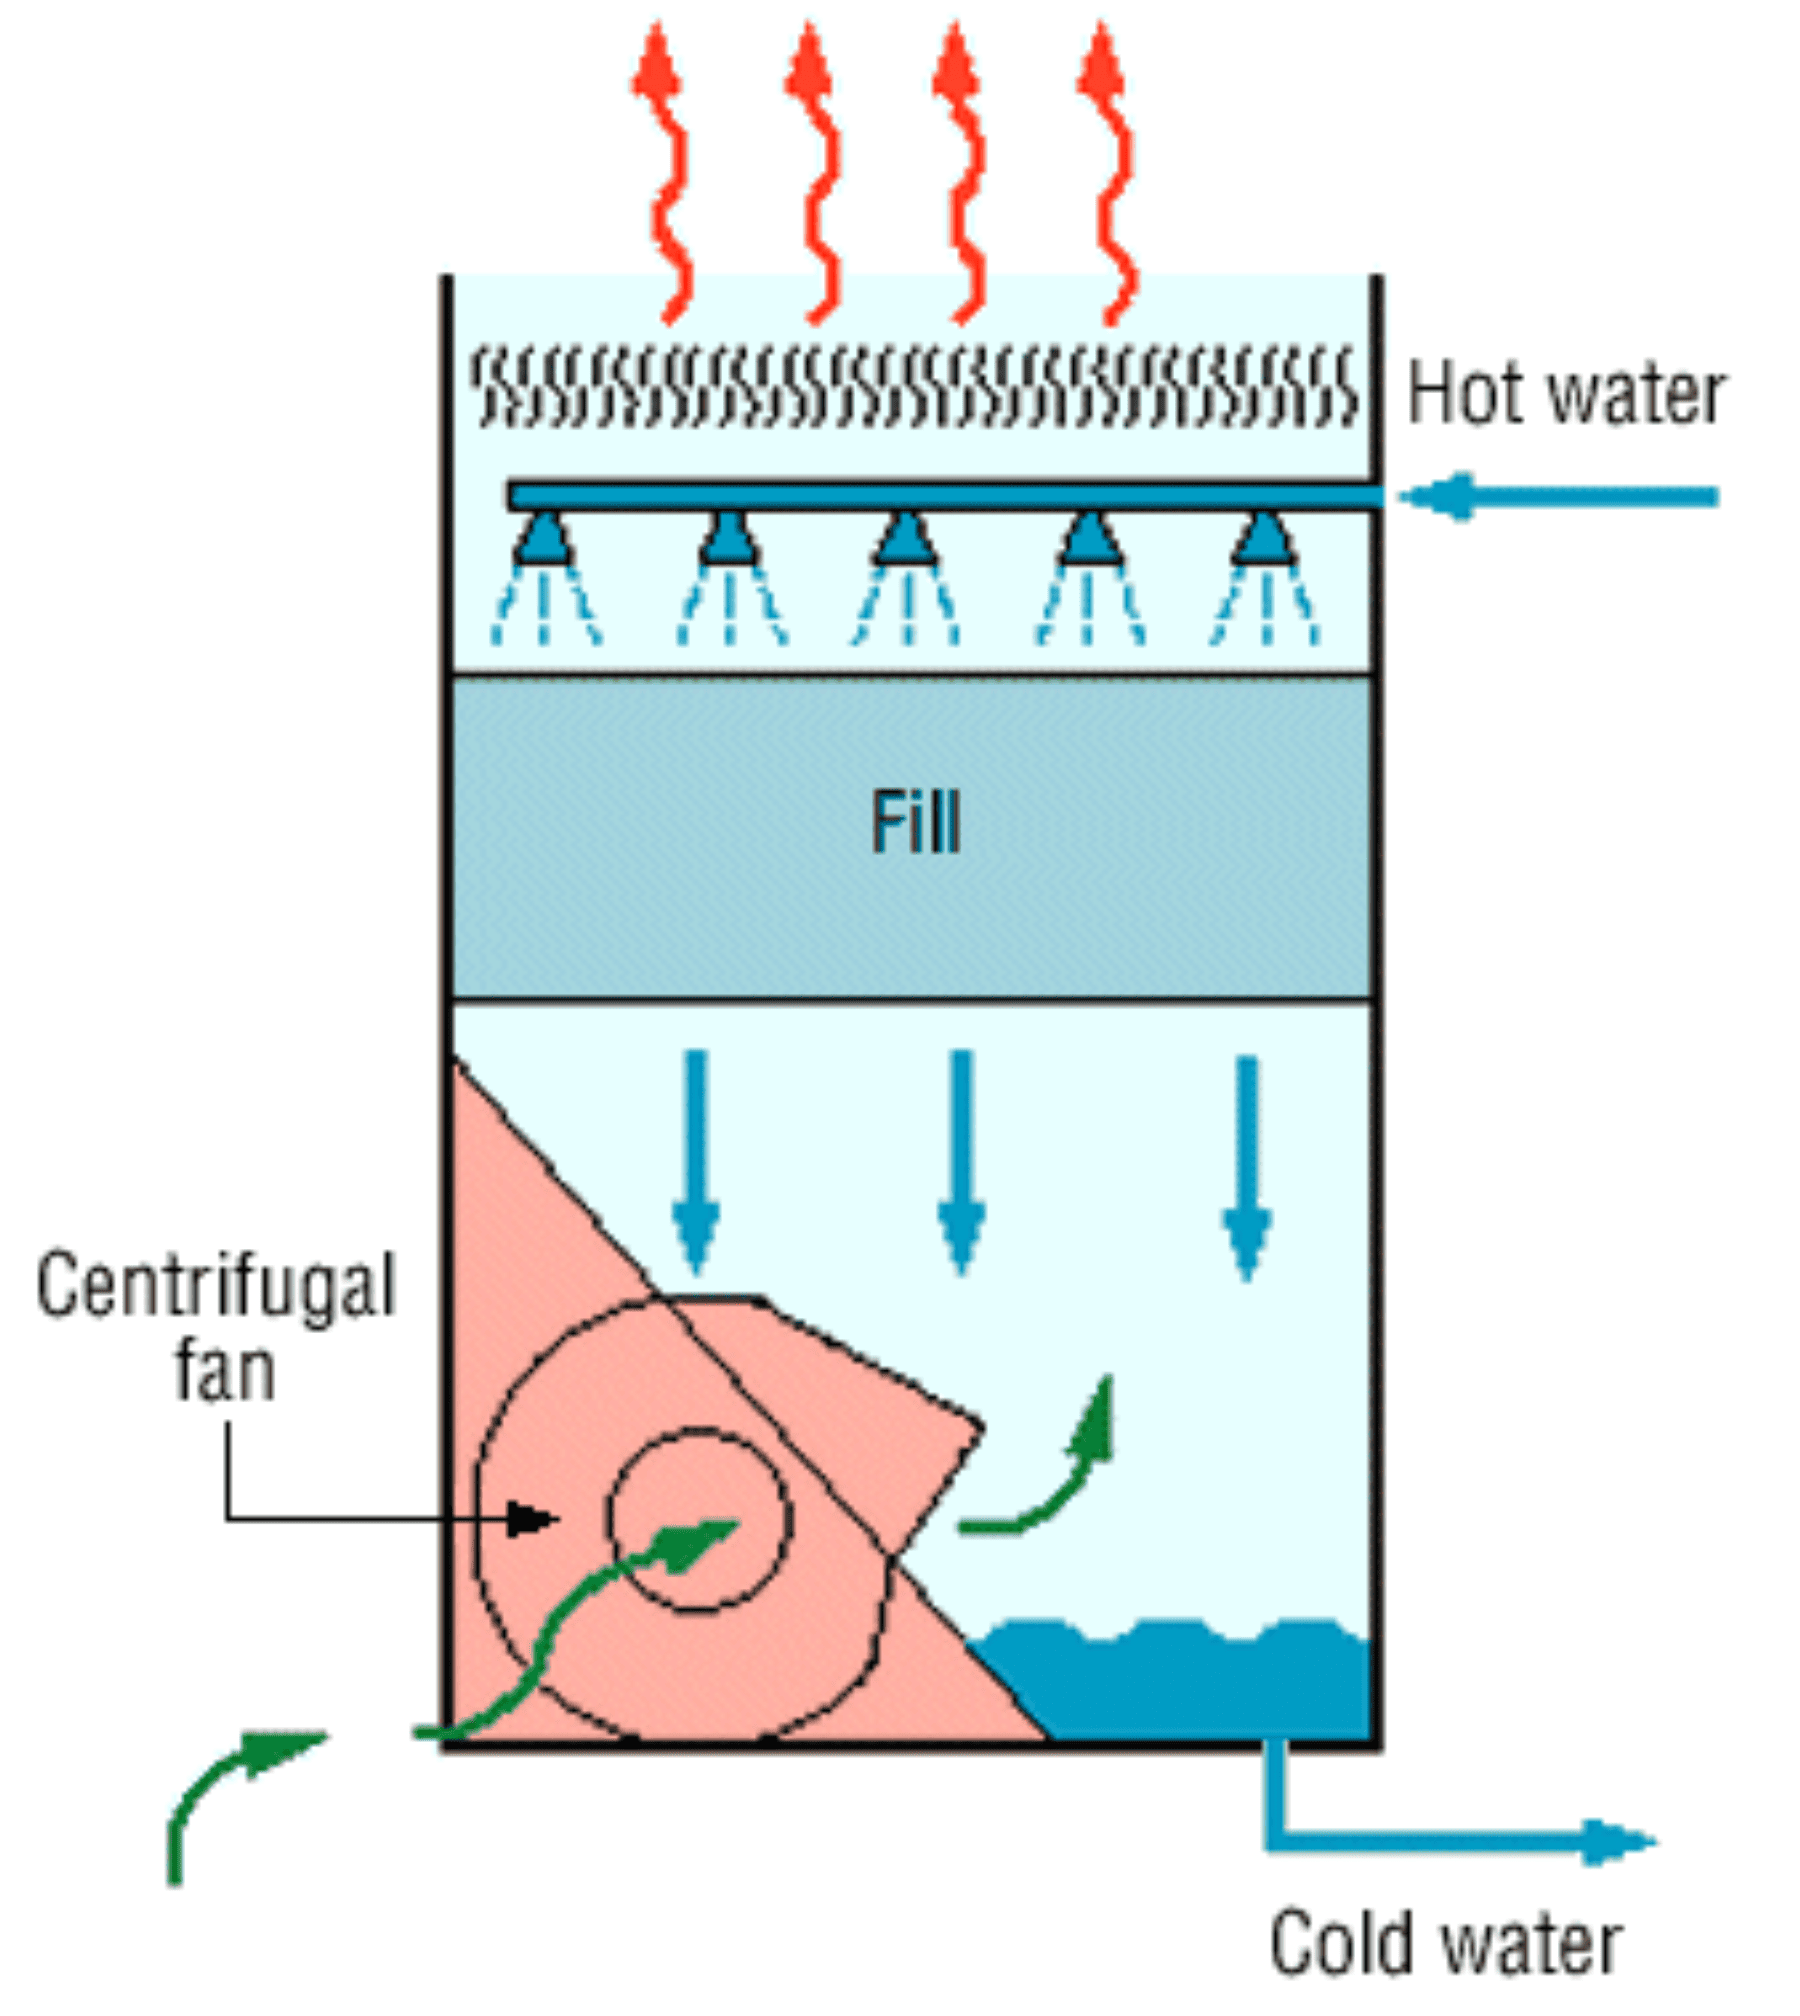
\includegraphics[width=0.6\textwidth]{Hinhve/doi_luu_cuong_buc.png}
    \caption{Tháp giải nhiệt đối lưu cưỡng bức \cite{unep2006coolingtower_en}}
    \label{fig:doi_luu_cuong_buc}
\end{figure}

Tháp giải nhiệt đối lưu cưỡng bức có nhiều ưu điểm nổi bật trong thiết kế và vận hành. Khả năng kiểm soát tốt lưu lượng không khí cho phép điều chỉnh chính xác hiệu suất làm mát theo nhu cầu thực tế. Loại tháp này ít bị ảnh hưởng bởi gió bên ngoài nhờ vào cơ chế đẩy không khí từ phía dưới, tạo ra dòng khí ổn định và không phụ thuộc vào điều kiện thời tiết. Việc bảo trì quạt cũng trở nên dễ dàng hơn do vị trí thuận tiện ở đáy tháp, giảm thời gian và chi phí bảo trì. Ngoài ra, thiết kế này còn mang lại sự phân bố không khí đều hơn trên toàn bộ diện tích tháp, đảm bảo hiệu quả truyền nhiệt tối ưu.

Tuy nhiên, loại tháp này cũng tồn tại những hạn chế nhất định. Tiêu thụ năng lượng cao hơn là nhược điểm chính do quạt phải làm việc chống lại áp suất tĩnh của cả tổng thể tháp, đòi hỏi công suất lớn hơn so với loại hút khí. Hiện tượng tái tuần hoàn khí nóng ẩm có thể xảy ra trong một số điều kiện đặc biệt, khi khí đã qua quá trình làm mát bị hút trở lại vào đầu vào của tháp, làm giảm hiệu quả tổng thể. Những yếu tố này dẫn đến chi phí vận hành tương đối cao hơn so với các loại tháp khác, đặc biệt trong các ứng dụng vận hành liên tục.

\subsubsection{Tháp giải nhiệt đối lưu hút}
Tháp giải nhiệt đối lưu hút sử dụng quạt để hút không khí ra khỏi tháp từ phía trên. Quạt được đặt ở đỉnh tháp, tạo ra lực hút để không khí được đưa vào từ các bên và đi ra từ trên \cite{johnson_mechanical_draft_2016}.

\begin{figure}[H]
    \centering
    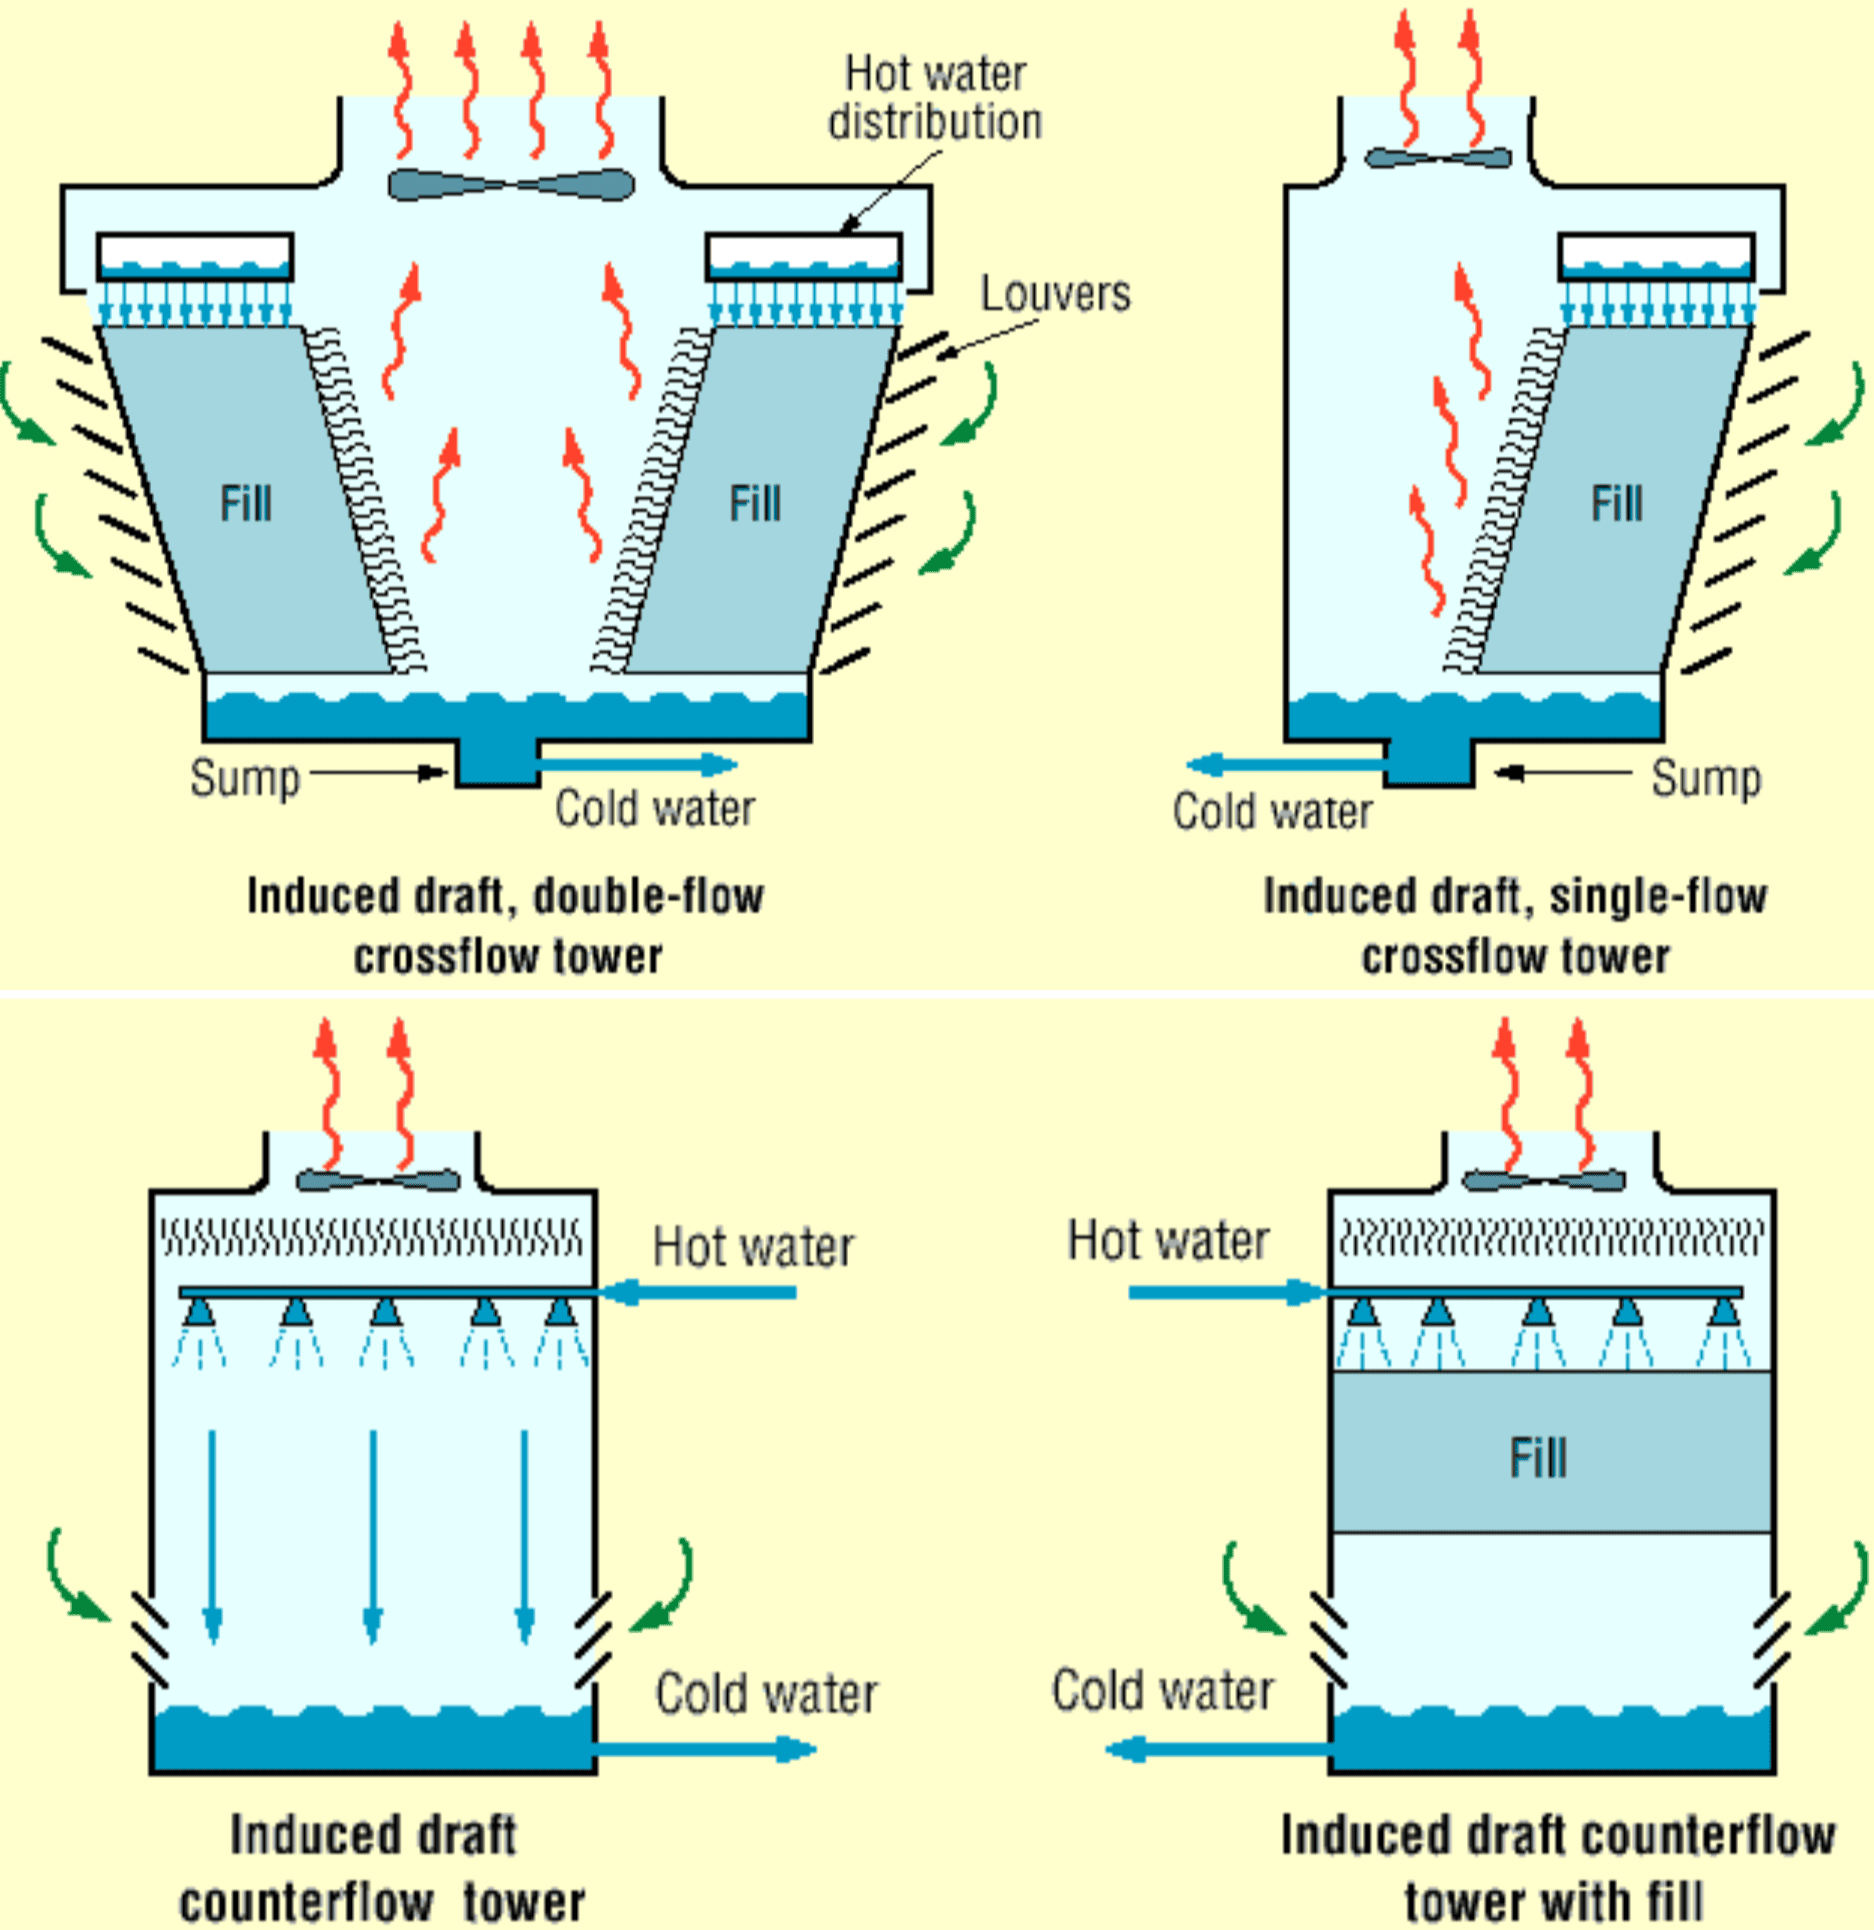
\includegraphics[width=0.9\textwidth]{Hinhve/doi_luu_hut.png}
    \caption{Một số kiểu tháp giải nhiệt đối lưu hút : Tháp giải nhiệt đối lưu ngược dòng (trên) và tháp giải nhiệt đối lưu dòng ngang (dưới) \cite{unep2006coolingtower_en}}
    \label{fig:doi_luu_hut}
\end{figure}

Tháp giải nhiệt đối lưu hút thể hiện những ưu thế vượt trội về hiệu quả năng lượng và chất lượng vận hành. Hiệu suất năng lượng cao hơn so với loại cưỡng bức là ưu điểm nổi bật nhất, do quạt chỉ cần vượt qua áp suất của phần đệm và không phải chống lại toàn bộ áp suất tĩnh của tháp. Hiện tượng tái tuần hoàn khí nóng ẩm cũng ít xảy ra hơn nhờ vào cơ chế hút khí từ trên xuống, tạo ra vận tốc khí thoát cao và giảm khả năng khí đã xử lý trở lại vào hệ thống. Sự phân bố nhiệt độ không khí đầu ra đều hơn cũng là một lợi thế quan trọng, giúp đảm bảo hiệu quả làm mát đồng đều trên toàn bộ diện tích. Đặc biệt, loại tháp này còn giúp giảm nguy cơ đóng băng ở các vùng khí hậu lạnh do khí nóng ẩm được hút ra nhanh chóng.

Mặt khác, loại tháp này cũng có những hạn chế riêng cần được cân nhắc. Việc bảo trì quạt trở nên khó khăn hơn do vị trí cao ở đỉnh tháp, đòi hỏi thiết bị chuyên dụng và kỹ năng an toàn cao của nhân viên bảo trì. Hệ thống cũng dễ bị ảnh hưởng bởi gió ngang, có thể làm thay đổi hướng dòng khí và ảnh hưởng đến hiệu suất. Cuối cùng, sự phân bố không khí vào có thể không đều do lực hút từ trên xuống, đặc biệt ở các vùng gần thành tháp, có thể tạo ra các vùng chết hoặc lưu lượng khí thấp.

\subsubsection{Tháp giải nhiệt thông gió tự nhiên}
Loại tháp này không sử dụng quạt mà dựa vào hiệu ứng ống khói tự nhiên. Không khí nóng nhẹ hơn sẽ tự động bốc lên, tạo ra dòng đối lưu tự nhiên \cite{patterson_natural_draft_cooling_2013}.

\begin{figure}[H]
    \centering
    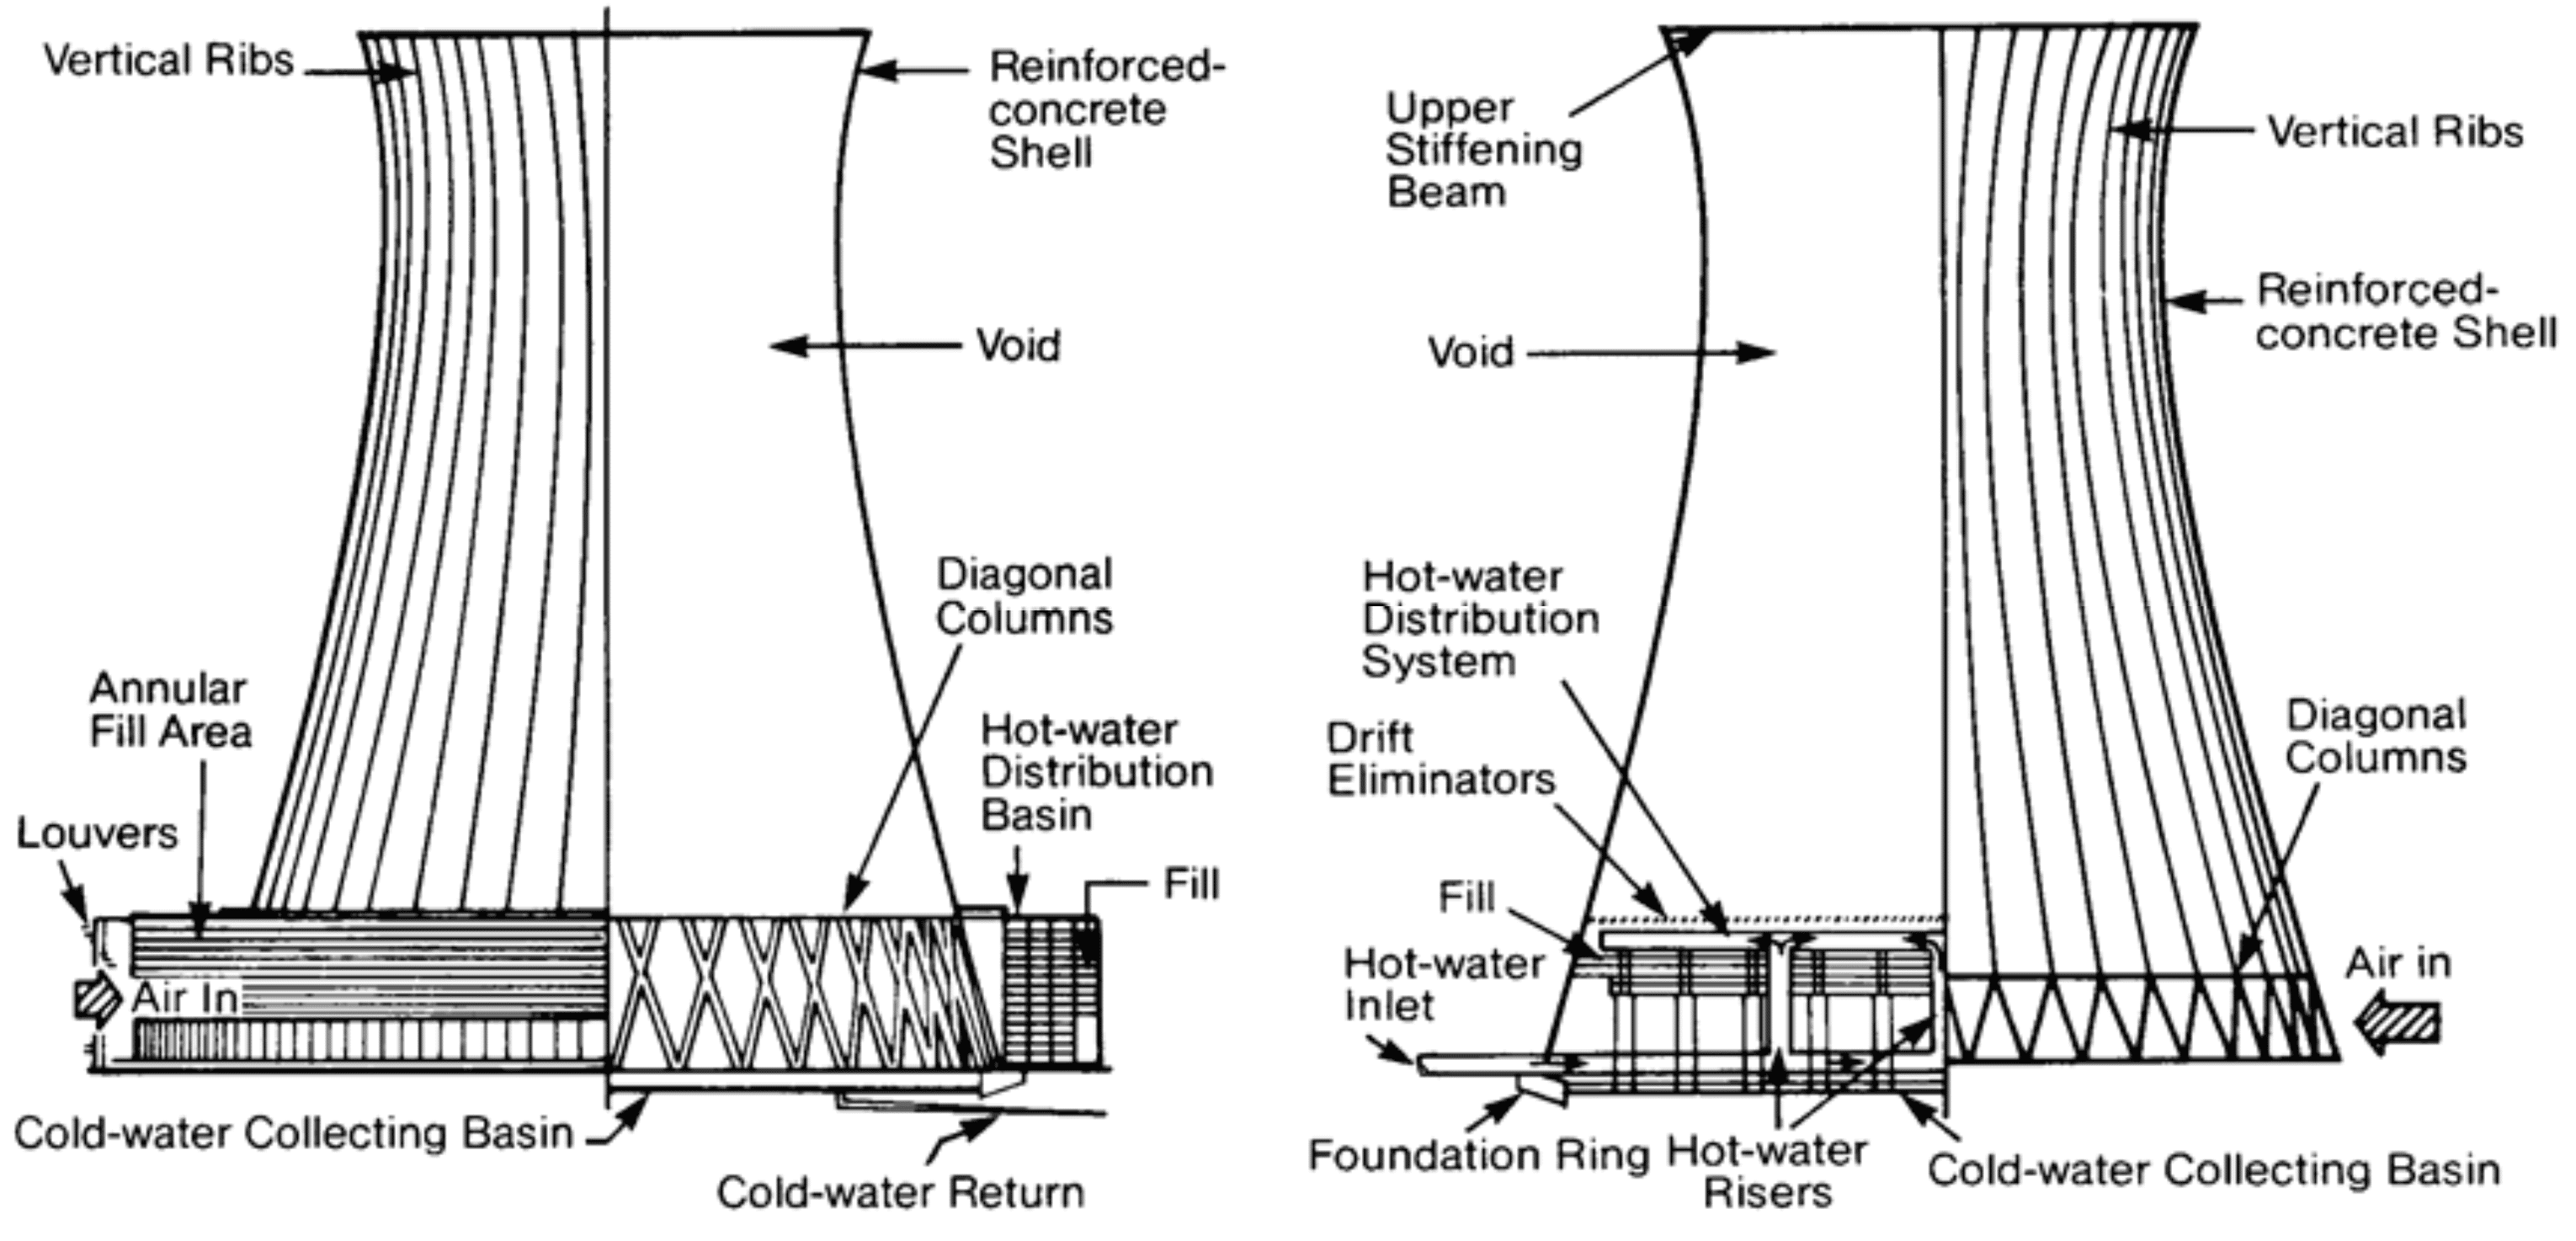
\includegraphics[width=1\textwidth]{Hinhve/thap_doi_luu.png}
    \caption{Hai dạng cấu hình chủ yếu của tháp giải nhiệt đối lưu tự nhiên: (trái) tháp dòng ngang, trong đó không khí lưu thông theo phương ngang so với dòng nước rơi; và (phải) tháp dòng ngược, trong đó không khí lưu thông theo phương ngược chiều với dòng nước \cite{unep2006coolingtower_en}}
    \label{fig:thap_doi_luu}
\end{figure}

Tháp giải nhiệt thông gió tự nhiên có những ưu điểm vượt trội về mặt kinh tế và môi trường. Loại tháp này không tiêu thụ năng lượng cho quạt, dẫn đến chi phí vận hành rất thấp và thân thiện với môi trường. Tiếng ồn được giảm thiểu đáng kể do không có thiết bị cơ khí hoạt động, tạo môi trường làm việc yên tĩnh. Độ tin cậy cao cũng là một ưu điểm quan trọng nhờ vào cấu trúc đơn giản với ít thiết bị cơ khí phức tạp, giảm nguy cơ hỏng hóc và nhu cầu bảo trì.

Tuy nhiên, loại tháp này cũng tồn tại những hạn chế đáng kể trong thiết kế và vận hành. Hiệu suất làm mát thường thấp hơn so với các loại tháp có quạt do phụ thuộc hoàn toàn vào dòng đối lưu tự nhiên. Kích thước tháp thường rất lớn để đảm bảo đủ diện tích trao đổi nhiệt, dẫn đến việc chiếm nhiều diện tích xây dựng. Hiệu suất hoạt động phụ thuộc mạnh vào điều kiện thời tiết như nhiệt độ, độ ẩm và tốc độ gió, khiến việc dự đoán và kiểm soát năng suất làm mát trở nên khó khăn.

\subsection{Phân loại theo kiểu tiếp xúc nước-không khí}
\label{sec:classification_by_contact_type}

\subsubsection{Tháp giải nhiệt tiếp xúc trực tiếp}
Trong loại tháp này, nước và không khí tiếp xúc trực tiếp với nhau. Nước được phun ra thành giọt hoặc tạo thành màng mỏng để tăng diện tích tiếp xúc.

Cơ chế truyền nhiệt trong tháp giải nhiệt tiếp xúc trực tiếp bao gồm ba quá trình đồng thời: truyền nhiệt hiện do chênh lệch nhiệt độ giữa nước và không khí, truyền nhiệt ẩn do bay hơi một phần nước vào không khí, và truyền khối do khuếch tán hơi nước vào không khí khô \cite{ashrae2020cooling}. Sự kết hợp của ba cơ chế này tạo nên hiệu quả làm mát vượt trội so với các phương pháp truyền nhiệt đơn thuần.

Loại tháp này được ứng dụng phổ biến trong các hệ thống HVAC, nhà máy điện và công nghiệp hóa chất nhờ hiệu suất cao và chi phí vận hành hợp lý.

\subsubsection{Tháp giải nhiệt tiếp xúc gián tiếp}
Nước cần làm mát được tuần hoàn trong hệ thống ống kín, không tiếp xúc trực tiếp với không khí. Việc trao đổi nhiệt diễn ra qua thành ống.

Tháp giải nhiệt tiếp xúc gián tiếp có những ưu điểm vượt trội về chất lượng nước và độ bền hệ thống. Nước không bị ô nhiễm do được cách ly hoàn toàn với môi trường bên ngoài, đồng thời không có hiện tượng mất nước do bay hơi. Điều này làm cho loại tháp này đặc biệt phù hợp với các ứng dụng yêu cầu nước có chất lượng cao như trong công nghiệp dược phẩm hoặc thực phẩm. Hơn nữa, hệ thống ít tạo cặn và ăn mòn do nước được bảo vệ trong môi trường kín.

Tuy nhiên, loại tháp này cũng có những hạn chế đáng kể. Hiệu suất làm mát thấp hơn so với loại tiếp xúc trực tiếp do thiếu cơ chế truyền nhiệt ẩn từ quá trình bay hơi. Chi phí đầu tư cao hơn đáng kể do cần hệ thống ống dẫn phức tạp và thiết bị trao đổi nhiệt chuyên dụng. Kích thước tháp cũng lớn hơn để đạt được cùng năng suất làm mát so với loại tiếp xúc trực tiếp.

\subsection{Phân loại theo vật liệu đệm}
\label{sec:classification_by_fill_material}

\subsubsection{Tháp giải nhiệt dạng phun}
Sử dụng các thanh gỗ hoặc nhựa được sắp xếp theo từng tầng để tạo ra nhiều bậc rơi cho nước. Khi nước rơi qua các bậc này, nó bị tách thành những giọt nhỏ, tăng diện tích tiếp xúc với không khí \cite{marriott_practical_thermal_2009}.

Tháp giải nhiệt dạng phun có những đặc điểm kỹ thuật phù hợp với nhiều điều kiện vận hành khác nhau. Loại tháp này đặc biệt phù hợp với nước có độ ô nhiễm cao do cấu trúc mở và không gian rộng giữa các thanh đệm. Việc vệ sinh và bảo trì trở nên dễ dàng nhờ thiết kế đơn giản và khả năng tiếp cận tốt. Khả năng chống tắc nghẽn vượt trội là một ưu điểm quan trọng, đặc biệt trong các môi trường có nhiều cặn bẩn hoặc chất rắn lơ lửng. Tuy nhiên, hiệu suất làm mát chỉ ở mức trung bình do diện tích tiếp xúc hạn chế so với các loại đệm hiện đại khác.

\subsubsection{Tháp giải nhiệt dạng màng}
Sử dụng các tấm nhựa định hình đặc biệt để tạo thành những màng nước mỏng chảy xuống. Điều này tạo ra diện tích tiếp xúc rất lớn giữa nước và không khí \cite{marriott_practical_thermal_2009}.

Tháp giải nhiệt dạng màng đại diện cho công nghệ tiên tiến nhất trong thiết kế đệm làm mát. Hiệu suất của loại tháp này là cao nhất trong các loại tháp giải nhiệt nhờ diện tích tiếp xúc riêng rất lớn giữa nước và không khí. Thiết kế tấm nhựa định hình đặc biệt tạo ra hàng nghìn màng nước mỏng, tối đa hóa quá trình truyền nhiệt và truyền khối. Tuy nhiên, loại đệm này đòi hỏi nước sạch với ít cặn bẩn để duy trì hiệu suất tối ưu. Nhược điểm chính là dễ bị tắc nghẽn nếu nước có độ ô nhiễm cao, đòi hỏi hệ thống xử lý nước nghiêm ngặt và bảo trì định kỳ tần suất cao.

\section{Các yếu tố ảnh hưởng đến hiệu suất tháp giải nhiệt}
\label{sec:factors_affecting_performance}

\subsection{Yếu tố khí tượng}
\label{sec:meteorological_factors}

\subsubsection{Nhiệt độ bầu ướt không khí}
Nhiệt độ bầu ướt là yếu tố quan trọng nhất quyết định hiệu suất của tháp giải nhiệt. Nó đại diện cho giới hạn lý thuyết thấp nhất mà nhiệt độ nước có thể đạt được \cite{ashrae2020cooling}.

Ảnh hưởng của nhiệt độ bầu ướt đến hiệu suất tháp giải nhiệt có tính chất quyết định. Khi nhiệt độ bầu ướt thấp, hiệu suất làm mát sẽ cao do chênh lệch nhiệt độ lớn giữa nước nóng và giới hạn làm mát lý thuyết. Chênh lệch giữa nhiệt độ nước ra và nhiệt độ bầu ướt được gọi là "approach" - một thông số quan trọng trong thiết kế tháp. Approach nhỏ cho thấy thiết kế tháp hiệu quả hơn, tuy nhiên điều này đồng nghĩa với chi phí đầu tư cao hơn do cần diện tích trao đổi nhiệt lớn hơn.

Biến đổi theo mùa của nhiệt độ bầu ướt tạo ra sự thay đổi đáng kể trong hiệu suất tháp giải nhiệt. Mùa đông với nhiệt độ bầu ướt thấp tạo điều kiện thuận lợi cho hiệu suất làm mát cao. Ngược lại, mùa hè với nhiệt độ bầu ướt cao làm giảm đáng kể hiệu suất làm mát. Đặc biệt, mùa mưa với độ ẩm không khí cao sẽ làm tăng nhiệt độ bầu ướt, từ đó hạn chế khả năng làm mát của tháp.

\subsubsection{Tốc độ và hướng gió}
Gió tự nhiên có thể tích cực hoặc tiêu cực đến hoạt động của tháp giải nhiệt:

Gió tự nhiên có ảnh hưởng đa chiều đến hoạt động của tháp giải nhiệt, vừa mang lại lợi ích vừa tạo ra thách thức. Về mặt tích cực, gió nhẹ giúp thổi bay khí nóng ẩm ra khỏi tháp một cách tự nhiên, tăng lưu lượng không khí qua tháp và giảm hiện tượng tái tuần hoàn khí đã qua xử lý. Điều này có thể cải thiện hiệu suất làm mát mà không cần tăng công suất quạt.

Tuy nhiên, gió cũng có thể gây ra những ảnh hưởng tiêu cực đáng kể. Gió mạnh có thể làm giảm lưu lượng không khí qua tháp do tạo ra áp suất ngược. Gió ngang đặc biệt có hại khi có thể tạo ra vùng áp suất âm ở một bên tháp, làm giảm hiệu suất tổng thể. Trong điều kiện gió bất lợi, hiện tượng tái tuần hoàn khí nóng ẩm có thể xảy ra nghiêm trọng, làm giảm đáng kể khả năng làm mát của hệ thống.

\subsection{Yếu tố thiết kế}
\label{sec:design_factors}

\subsubsection{Tỷ lệ L/G (Liquid to Gas ratio)}
Tỷ lệ giữa lưu lượng khối lượng nước và không khí là một thông số thiết kế quan trọng \cite{marriott_practical_thermal_2009}:

\begin{equation}
    L/G = \frac{\dot{m}_{\text{nước}}}{\dot{m}_{\text{không khí}}}
\end{equation}

Ảnh hưởng của tỷ lệ L/G đến hiệu suất và tiêu thụ năng lượng có tính chất đánh đổi quan trọng trong thiết kế tháp. Tỷ lệ L/G cao sẽ mang lại hiệu suất làm mát cao do tăng cường truyền nhiệt, nhưng đồng thời đòi hỏi tiêu thụ năng lượng quạt lớn để duy trì lưu lượng không khí cần thiết. Ngược lại, tỷ lệ L/G thấp giúp tiết kiệm năng lượng đáng kể nhưng với cái giá là hiệu suất làm mát giảm. Trong thực tế, tỷ lệ tối ưu thường được thiết kế trong khoảng 1.0 đến 1.5 để cân bằng giữa hiệu suất và tiết kiệm năng lượng.

\subsubsection{Chiều cao và diện tích tháp}
Các thông số hình học của tháp giải nhiệt có ảnh hưởng trực tiếp đến hiệu suất và đặc tính vận hành \cite{cti_cooling_towers_2011}. Chiều cao tháp quyết định thời gian tiếp xúc giữa nước và không khí - tăng chiều cao sẽ cải thiện hiệu suất do thời gian trao đổi nhiệt dài hơn. Diện tích mặt cắt của tháp quyết định tốc độ không khí đi qua, ảnh hưởng trực tiếp đến hiệu suất truyền nhiệt và mức độ rơi nước. Thể tích đệm cũng đóng vai trò quan trọng khi tăng thể tích đệm sẽ tăng diện tích tiếp xúc riêng, từ đó nâng cao hiệu quả truyền nhiệt tổng thể.

\subsection{Yếu tố vận hành}
\label{sec:operational_factors}

\subsubsection{Chất lượng nước}
\label{sec:water_quality}

Chất lượng nước tuần hoàn đóng vai trò then chốt trong việc duy trì hiệu suất và kéo dài tuổi thọ vận hành của tháp giải nhiệt \cite{epa_cooling_tower_guide_2017,ashrae2020cooling}. Nước sử dụng trong hệ thống thường chứa nhiều tạp chất vô cơ, hữu cơ và hóa chất xử lý, mỗi loại đều có thể gây ảnh hưởng tiêu cực đến quá trình trao đổi nhiệt và độ bền của thiết bị.

\textbf{Độ cứng của nước} là một yếu tố quan trọng, phản ánh nồng độ các ion canxi (Ca$^{2+}$) và magiê (Mg$^{2+}$). Nồng độ cao các ion này dễ dẫn đến sự hình thành cặn bám trên bề mặt khối đệm và các bộ phận trao đổi nhiệt, làm giảm diện tích tiếp xúc hiệu quả giữa nước và không khí, từ đó suy giảm hệ số truyền nhiệt tổng thể \cite{unep2006coolingtower_en}. Để khắc phục, cần áp dụng các biện pháp xử lý làm mềm nước hoặc thực hiện vệ sinh định kỳ theo lịch trình nghiêm ngặt.

\textbf{Chất rắn lơ lửng} (Suspended Solids – SS) trong nước cũng là nguyên nhân gây ra nhiều vấn đề vận hành nghiêm trọng. Các hạt rắn này có xu hướng tích tụ thành cặn bẩn, gây tắc nghẽn hệ thống phân phối nước, dẫn đến phân bố nước không đồng đều trên bề mặt đệm, làm giảm hiệu quả trao đổi nhiệt \cite{ashrae2020cooling}. Hậu quả là tăng tần suất bảo trì, gia tăng chi phí vận hành và thời gian ngừng hoạt động ngoài kế hoạch.

\textbf{Thành phần hóa học của nước} cần được kiểm soát chặt chẽ. Clo dư (residual chlorine) với nồng độ cao có thể gây ăn mòn các bộ phận kim loại, trong khi giá trị pH không phù hợp sẽ ảnh hưởng bất lợi đến cả kim loại và vật liệu phi kim của tháp \cite{epa_cooling_tower_guide_2017}. Do đó, việc giám sát và điều chỉnh các thông số hóa học của nước đầu vào là yêu cầu bắt buộc nhằm đảm bảo tuổi thọ thiết bị, hạn chế sự cố và duy trì hiệu suất vận hành tối ưu.

\subsubsection{Tần suất và chất lượng bảo trì}
Bảo trì tháp giải nhiệt đòi hỏi một chương trình toàn diện bao gồm nhiều hoạt động chuyên biệt \cite{epa_cooling_tower_guide_2017}. Vệ sinh đệm phải được thực hiện định kỳ để loại bỏ cặn bẩn, tảo và vi khuẩn tích tụ theo thời gian. Kiểm tra quạt bao gồm các hoạt động cân bằng, bôi trơn và thay thế các bộ phận khi cần thiết để đảm bảo hoạt động ổn định. Hệ thống phân phối nước cần được duy trì để đảm bảo sự phân phối đều trên toàn bộ diện tích đệm. Cuối cùng, xử lý nước là hoạt động liên tục bao gồm kiểm soát pH, độ cứng và nồng độ chất khử trùng trong giới hạn cho phép.

\section{Phương pháp đánh giá hiệu suất tháp giải nhiệt}
\label{sec:performance_evaluation_methods}

\subsection{Các chỉ số hiệu suất quan trọng}
\label{sec:key_performance_indicators}

\subsubsection{Chỉ số hiệu suất chuẩn hóa}
Ngoài hiệu suất nhiệt cơ bản đã trình bày trong phần \ref{sec:cooling_capacity_efficiency}, việc đánh giá hiệu suất tháp giải nhiệt còn sử dụng các chỉ số chuẩn hóa để so sánh với điều kiện thiết kế và tiêu chuẩn ngành:

\begin{equation}
    \eta_{\text{norm}} = \frac{\eta_{\text{thực tế}}}{\eta_{\text{thiết kế}}} \times 100\%
\end{equation}

Chỉ số này cho phép đánh giá mức độ suy giảm hiệu suất so với điều kiện thiết kế ban đầu. Giá trị $\eta_{\text{norm}} < 85\%$ thường chỉ báo cần bảo trì hoặc kiểm tra hệ thống.

\subsubsection{Hệ số truyền nhiệt tổng thể}
Hệ số này phản ánh khả năng truyền nhiệt của toàn bộ hệ thống \cite{marriott_practical_thermal_2009}:

\begin{equation}
    U = \frac{Q}{A \cdot \Delta T_{\text{lm}}}
\end{equation}
Trong đó:
\begin{itemize}
    \item $U$: Hệ số truyền nhiệt tổng thể ($\mathrm{W/(m^2 \cdot K)}$)
    \item $Q$: Công suất truyền nhiệt ($\mathrm{W}$)
    \item $A$: Diện tích truyền nhiệt ($\mathrm{m^2}$)
    \item $\Delta T_{\text{lm}}$: Chênh lệch nhiệt độ trung bình logarit ($\mathrm{K}$)
\end{itemize}
Hệ số $U$ là thước đo quan trọng để đánh giá hiệu quả trao đổi nhiệt của toàn bộ hệ thống.

\subsubsection{Số đơn vị truyền nhiệt (Number of Transfer Units - NTU)}
NTU (Number of Transfer Units) là một thông số không thứ nguyên rất quan trọng trong thiết kế tháp giải nhiệt. Thông số này phản ánh mức độ hiệu quả của quá trình truyền khối (trao đổi nhiệt và ẩm) giữa nước và không khí bên trong tháp. Giá trị NTU càng lớn thì khả năng truyền khối càng cao, đồng nghĩa với hiệu suất làm mát tốt hơn. NTU cũng là cơ sở kỹ thuật để xác định kích thước tối ưu của tháp giải nhiệt, đảm bảo đáp ứng yêu cầu vận hành thực tế.

\begin{equation}
    \text{NTU} = \frac{K \cdot a \cdot V}{L}
\end{equation}
Trong đó:
\begin{itemize}
    \item $K$: Hệ số truyền khối tổng thể
    \item $a$: Diện tích riêng của đệm ($\mathrm{m^2/m^3}$)
    \item $V$: Thể tích đệm ($\mathrm{m^3}$)
    \item $L$: Lưu lượng nước ($\mathrm{kg/s}$)
\end{itemize}

\subsection{Phương pháp đo đạc và thử nghiệm}
\label{sec:measurement_testing_methods}

\subsubsection{Tiêu chuẩn thử nghiệm}

Việc đánh giá hiệu suất của tháp giải nhiệt cần được thực hiện theo các tiêu chuẩn quốc tế nhằm đảm bảo tính khách quan, độ tin cậy và khả năng so sánh kết quả giữa các hệ thống khác nhau. 

\textbf{Tiêu chuẩn ASME PTC~23} \cite{ashrae2020cooling} đưa ra một khung hướng dẫn toàn diện cho việc thử nghiệm và đánh giá hiệu suất của tháp giải nhiệt. Tiêu chuẩn này quy định cụ thể phương pháp thử nghiệm chuẩn, các điều kiện vận hành tiêu chuẩn cần thiết, cũng như các yêu cầu về thu thập, xử lý và phân tích dữ liệu. Đồng thời, ASME PTC~23 cũng nêu rõ các tiêu chí để hiệu chỉnh số liệu và đánh giá sai số đo, nhằm đảm bảo kết quả phản ánh chính xác đặc tính vận hành thực tế của tháp.

\textbf{Tiêu chuẩn CTI ATC-105} \cite{cti_cooling_towers_2011} là tiêu chuẩn quốc tế chuyên biệt hướng dẫn chi tiết quy trình thử nghiệm nghiệm thu hiệu suất tháp giải nhiệt nước. Tiêu chuẩn này quy định rõ các điều kiện thử nghiệm, phương pháp đo lường các thông số vận hành chính (nhiệt độ, lưu lượng nước, lưu lượng không khí, điều kiện môi trường), yêu cầu về độ chính xác và hiệu chuẩn thiết bị đo, cũng như các bước xử lý và phân tích số liệu để xác định hiệu suất thực tế của tháp. CTI ATC-105 nhấn mạnh việc kiểm soát sai số đo và đánh giá độ không đảm bảo đo, đồng thời yêu cầu thực hiện kiểm tra lặp lại để đảm bảo tính tin cậy và khả năng tái lập của kết quả. Tiêu chuẩn này thường được áp dụng trong giai đoạn nghiệm thu, bàn giao thiết bị mới hoặc sau khi cải tạo lớn, là cơ sở kỹ thuật để so sánh hiệu suất thực tế với các thông số cam kết của nhà sản xuất, và là tài liệu tham chiếu bắt buộc trong các hợp đồng EPC hoặc bảo hành hiệu suất.

\subsubsection{Hệ thống đo lường và thu thập dữ liệu}
Hệ thống đo lường cho đánh giá hiệu suất tháp giải nhiệt phải đáp ứng các yêu cầu kỹ thuật nghiêm ngặt về độ chính xác và độ tin cậy. Đo nhiệt độ sử dụng cảm biến nhiệt điện trở (RTD) loại Pt100 với độ chính xác $\pm 0.1^\circ\mathrm{C}$ cho các điểm đo quan trọng, đặc biệt tại đầu vào và đầu ra nước. Việc bố trí nhiều điểm đo tại mỗi vị trí và tính giá trị trung bình giúp giảm thiểu sai số do phân bố nhiệt độ không đồng đều.

Đo lưu lượng nước áp dụng lưu lượng kế điện từ\footnote{Lưu lượng kế điện từ (Electromagnetic flowmeter): thiết bị đo lưu lượng chất lỏng dựa trên nguyên lý cảm ứng điện từ, thường dùng cho nước dẫn điện.} với độ chính xác $\pm 1\%$ của thang đo, đặt tại vị trí có dòng chảy ổn định, tránh các vùng nhiễu động. Lưu lượng không khí được xác định thông qua đo tốc độ tại nhiều điểm trên mặt cắt tháp bằng anemometer nhiệt\footnote{Anemometer nhiệt (Hot-wire anemometer): thiết bị đo tốc độ gió dựa trên sự thay đổi điện trở của dây nung khi không khí đi qua.} và tích phân trên toàn bộ diện tích.

Hệ thống thu thập dữ liệu tự động với tần suất lấy mẫu $1{-}5$ Hz đảm bảo nắm bắt được các biến động ngắn hạn, đồng thời tích hợp bộ lọc nhiễu và thuật toán xác thực dữ liệu để loại bỏ các giá trị bất thường.

\subsection{Phân tích dữ liệu và đánh giá kết quả}
\label{sec:data_analysis_evaluation}

\subsubsection{Xử lý và chuẩn hóa dữ liệu}
Dữ liệu thô từ hệ thống đo lường cần được xử lý qua các bước chuẩn hóa để đảm bảo chất lượng phân tích. Thuật toán phát hiện ngoại lệ sử dụng phương pháp thống kê (Z-score hoặc IQR) \cite{zscore_iqr_stat} để loại bỏ các giá trị nằm ngoài khoảng tin cậy $99.7\%$. Bộ lọc Kalman\footnote{Bộ lọc Kalman (Kalman filter): thuật toán lọc tối ưu dùng để ước lượng trạng thái của hệ động lực tuyến tính từ dữ liệu đo nhiễu, thường được ứng dụng để làm mịn và dự báo chuỗi số liệu thời gian.} được áp dụng để làm mịn dữ liệu nhiệt độ, trong khi bộ lọc trung bình trượt có trọng số được sử dụng cho dữ liệu lưu lượng.

Hiệu chuẩn dữ liệu theo điều kiện chuẩn là bước thiết yếu để so sánh hiệu suất giữa các thời điểm khác nhau. Các thông số được chuẩn hóa về điều kiện nhiệt độ bầu ướt thiết kế ($T_{wb,design} = 27^\circ\mathrm{C}$) và tải nhiệt định mức theo công thức hiệu chỉnh của CTI.

\subsubsection{Phân tích thống kê và dự báo xu hướng}
Phân tích chuỗi thời gian áp dụng mô hình ARIMA\footnote{Mô hình ARIMA (AutoRegressive Integrated Moving Average): là mô hình dự báo chuỗi thời gian kết hợp ba thành phần: tự hồi quy (AR), sai phân (I) và trung bình trượt (MA), thường được sử dụng để phân tích và dự báo các dữ liệu có tính chu kỳ hoặc xu hướng.} \cite{box_jenkins_arima} để xác định xu hướng suy giảm hiệu suất dài hạn và dự báo nhu cầu bảo trì. Hệ số tương quan Pearson\footnote{Hệ số tương quan Pearson: $r = \frac{\sum_{i=1}^{n}(x_i - \bar{x})(y_i - \bar{y})}{\sqrt{\sum_{i=1}^{n}(x_i - \bar{x})^2}\sqrt{\sum_{i=1}^{n}(y_i - \bar{y})^2}}$ với $x_i, y_i$ là các giá trị quan sát, $\bar{x}, \bar{y}$ là giá trị trung bình. Hệ số $r$ nằm trong khoảng $[-1, +1]$, với $|r| > 0.7$ được coi là tương quan mạnh \cite{stull2011meteorology}.} được tính toán giữa hiệu suất tháp và các biến môi trường (nhiệt độ bầu ướt, tốc độ gió, tải nhiệt) để định lượng mức độ ảnh hưởng của từng yếu tố.

Phân tích hồi quy đa biến xây dựng mô hình dự báo hiệu suất dạng:
\begin{equation}
    \eta = \beta_0 + \beta_1 T_{wb} + \beta_2 Q_{load} + \beta_3 v_{wind} + \varepsilon
\end{equation}
trong đó các hệ số $\beta_i$ được ước lượng bằng phương pháp bình phương tối thiểu, cho phép dự báo hiệu suất trong các điều kiện vận hành khác nhau.

\subsubsection{Đánh giá kết quả và khuyến nghị kỹ thuật}
Báo cáo đánh giá hiệu suất tuân thủ cấu trúc chuẩn gồm: (1) Tóm tắt điều kiện thử nghiệm và phương pháp đo; (2) Bảng tổng hợp các chỉ số hiệu suất so với giá trị thiết kế; (3) Biểu đồ xu hướng hiệu suất theo thời gian; (4) Phân tích nguyên nhân sai lệch; (5) Ma trận đánh giá rủi ro vận hành.

Khuyến nghị kỹ thuật được phân loại theo mức độ ưu tiên: \textbf{Khẩn cấp} (hiệu suất < 70\% thiết kế) yêu cầu dừng vận hành ngay lập tức; \textbf{Cao} (70-85\%) cần bảo trì trong vòng 7 ngày; \textbf{Trung bình} (85-95\%) lập kế hoạch bảo trì trong tháng; \textbf{Thấp} (>95\%) duy trì theo lịch định kỳ. Mỗi khuyến nghị kèm theo ước tính chi phí và thời gian thực hiện.

\section{Ứng dụng IoT trong giám sát tháp giải nhiệt}
\label{sec:iot_applications_cooling_towers}

\subsection{Xu hướng số hóa trong công nghiệp}
\label{sec:digitalization_trends}

\subsubsection{Industry 4.0 và Internet of Things}
Cuộc cách mạng công nghiệp 4.0 đang thúc đẩy việc số hóa các quy trình công nghiệp, trong đó IoT đóng vai trò quan trọng trong việc kết nối và giám sát thiết bị \cite{zhang2022iot}. Đối với tháp giải nhiệt, IoT mang lại nhiều lợi ích:

Kết nối thông minh trong hệ thống IoT cho tháp giải nhiệt mang lại khả năng giám sát liên tục 24/7 mà không cần can thiệp của con người, thu thập dữ liệu đa thông số đồng thời từ nhiều cảm biến khác nhau \cite{statista2023iot}. Hệ thống có thể truyền dữ liệu thời gian thực qua mạng không dây đến trung tâm điều khiển và tích hợp hoàn toàn với hệ thống quản lý tòa nhà để tối ưu hóa tổng thể.

Phân tích dữ liệu lớn đóng vai trò quan trọng trong việc khai thác giá trị từ khối lượng dữ liệu khổng lồ được thu thập liên tục \cite{cisco2023iot}. Hệ thống có khả năng phát hiện các mẫu và xu hướng ẩn trong dữ liệu, dự báo chính xác hiệu suất và nhu cầu bảo trì, đồng thời tối ưu hóa vận hành dựa trên các thuật toán học máy tiên tiến.

\subsubsection{Lợi ích kinh tế của giám sát IoT}
Lợi ích kinh tế từ việc áp dụng giám sát IoT cho tháp giải nhiệt rất đáng kể và có thể đo lường được \cite{mckinsey2023digital}. Về tiết kiệm chi phí vận hành, hệ thống có thể giảm $10{-}30\%$ tiêu thụ năng lượng thông qua tối ưu hóa thông minh, giảm $25{-}50\%$ chi phí bảo trì nhờ khả năng bảo trì dự báo, tăng $15{-}25\%$ tuổi thọ thiết bị qua giám sát liên tục và giảm đáng kể thời gian downtime không kế hoạch.

Cải thiện hiệu quả vận hành là một lợi ích quan trọng khác của hệ thống IoT. Độ chính xác của phép đo và điều khiển được nâng cao đáng kể, khả năng phản ứng nhanh với những thay đổi trong điều kiện vận hành được cải thiện, tối ưu hóa theo thời gian thực trở thành khả thi, và hệ thống có thể tích hợp mượt mà với các hệ thống điều khiển tự động khác.

\section{Thực trạng và công nghệ hiện tại trong giám sát tháp giải nhiệt}
\label{sec:current_state_technologies}

\subsection{Phân tích thực trạng giám sát hiện tại}
\label{sec:current_monitoring_state}

Trong bối cảnh công nghiệp hiện tại, đa số các hệ thống tháp giải nhiệt vẫn được vận hành theo phương pháp truyền thống với mức độ tự động hóa và giám sát hạn chế \cite{wang2023smart}. Phương pháp giám sát chủ yếu dựa vào kiểm tra định kỳ bằng nhân lực, sử dụng các thiết bị đo đơn lẻ không kết nối mạng, và ghi chép dữ liệu thủ công. Cách tiếp cận này không chỉ tốn kém nhân lực mà còn dẫn đến việc phát hiện chậm các vấn đề vận hành, từ đó ảnh hưởng tiêu cực đến hiệu suất tổng thể và tuổi thọ thiết bị.

Theo nghiên cứu của McKinsey \cite{mckinsey2023digital}, chỉ có khoảng $25{-}30\%$ các cơ sở công nghiệp trên toàn cầu đã triển khai hệ thống giám sát tự động cho các thiết bị trao đổi nhiệt, trong đó tháp giải nhiệt chiếm tỷ lệ thấp hơn do tính phức tạp của môi trường vận hành. Tại các quốc gia đang phát triển như Việt Nam, tỷ lệ này còn thấp hơn đáng kể, phần lớn do hạn chế về ngân sách đầu tư, thiếu nhân lực chuyên môn và chưa có chính sách khuyến khích rõ ràng từ phía nhà nước \cite{vietnam2021energy}.

Thách thức lớn nhất trong việc áp dụng hệ thống giám sát hiện đại là sự thiếu hiểu biết về lợi ích kinh tế dài hạn từ phía các nhà quản lý. Nhiều doanh nghiệp vẫn tập trung vào chi phí đầu tư ban đầu mà chưa tính toán đầy đủ lợi ích từ việc tiết kiệm năng lượng, giảm chi phí bảo trì và tăng tuổi thọ thiết bị \cite{iea2023digitalization}. Điều này dẫn đến tình trạng nhiều tháp giải nhiệt hoạt động không hiệu quả, tiêu tốn nhiều năng lượng hơn cần thiết và thường xuyên gặp sự cố do thiếu giám sát kịp thời.

\subsection{Công nghệ cảm biến và vi điều khiển}
\label{sec:sensor_microcontroller_tech}

Sự phát triển nhanh chóng của công nghệ cảm biến trong những năm gần đây đã mở ra nhiều cơ hội nâng cao chất lượng giám sát và điều khiển tháp giải nhiệt. Các cảm biến nhiệt độ hiện đại, chẳng hạn như DS18B20 và DHT22, không chỉ có độ chính xác cao mà còn đáp ứng tốt yêu cầu vận hành trong môi trường công nghiệp khắc nghiệt \cite{ashrae2020cooling}. Cảm biến DS18B20 có độ chính xác điển hình $\pm 0.5^\circ\mathrm{C}$ trong khoảng $-10^\circ\mathrm{C}$ đến $+85^\circ\mathrm{C}$, dải đo mở rộng từ $-55^\circ\mathrm{C}$ đến $+125^\circ\mathrm{C}$, phù hợp cho đo nhiệt độ nước tuần hoàn trong tháp \cite{datasheet_DS18B20}. Cảm biến DHT22 ngoài khả năng đo nhiệt độ với độ chính xác tương đương, còn có thể đo độ ẩm tương đối với sai số điển hình $\pm 2\%$ đến $\pm 5\%$ RH trong khoảng $0$--$100\%$ RH, hữu ích cho việc xác định nhiệt độ bầu ướt \cite{datasheet_DHT22}.

Về vi điều khiển, dòng ESP32 của Espressif đã trở thành lựa chọn phổ biến trong các ứng dụng IoT công nghiệp nhờ khả năng tích hợp Wi-Fi và Bluetooth, bộ xử lý hai nhân với xung nhịp lên đến 240 MHz, tài nguyên bộ nhớ RAM tích hợp khoảng 520 KB, cùng chi phí hợp lý \cite{Espressif_ESP32_technical_reference,statista2023iot}. Vi điều khiển này có thể thu thập đồng thời dữ liệu từ nhiều cảm biến, thực hiện các tính toán cơ bản tại thiết bị (ví dụ: tính toán nhiệt độ bầu ướt, hiệu suất làm mát) và truyền dữ liệu thời gian thực tới hệ thống giám sát trung tâm. Khả năng lập trình linh hoạt cho phép tùy chỉnh thuật toán xử lý dữ liệu phù hợp với từng ứng dụng cụ thể.

Tuy nhiên, việc triển khai các thiết bị này trong môi trường tháp giải nhiệt đòi hỏi xem xét kỹ các yếu tố bảo vệ phần cứng. Độ ẩm cao, dao động nhiệt độ và sự hiện diện của hóa chất xử lý nước (như clo dư hoặc chất diệt tảo) có thể làm giảm độ tin cậy và tuổi thọ thiết bị \cite{epa_cooling_tower_guide_2017}. Do đó, việc thiết kế vỏ bảo vệ đạt tiêu chuẩn chống nước/bụi (ví dụ: IP65 hoặc cao hơn) và sử dụng vật liệu chống ăn mòn là các yếu tố then chốt trong giai đoạn thiết kế và triển khai hệ thống.

\subsection{Giao thức truyền thông và quản lý dữ liệu}
\label{sec:communication_protocols}

Lựa chọn giao thức truyền thông phù hợp đóng vai trò quyết định đến hiệu quả và độ tin cậy của hệ thống giám sát. MQTT (Message Queuing Telemetry Transport) đã được chứng minh là một giao thức hiệu quả cho các ứng dụng IoT trong môi trường công nghiệp, đặc biệt phù hợp với việc truyền dữ liệu từ tháp giải nhiệt do khả năng hoạt động ổn định với băng thông thấp và độ trễ nhỏ \cite{cisco2023iot}.

Về quản lý dữ liệu, các hệ thống cơ sở dữ liệu thời gian như InfluxDB đang được sử dụng rộng rãi để lưu trữ và xử lý dữ liệu cảm biến do khả năng tối ưu hóa cho việc ghi và truy vấn dữ liệu theo chuỗi thời gian \cite{li2023ai}. Điều này đặc biệt quan trọng đối với hệ thống giám sát tháp giải nhiệt, nơi dữ liệu được thu thập liên tục và cần được phân tích để nhận diện xu hướng và dự báo sự cố.

Việc tích hợp với các nền tảng cloud computing như AWS IoT, Google Cloud IoT hoặc Microsoft Azure IoT cũng mang lại nhiều lợi ích về khả năng mở rộng, bảo mật và phân tích dữ liệu nâng cao \cite{google2023datacenter,microsoft2023azure}. Tuy nhiên, các tổ chức cần cân nhắc giữa lợi ích của cloud computing và các yêu cầu về bảo mật dữ liệu, đặc biệt trong các ứng dụng liên quan đến hạ tầng quan trọng.

\subsection{Xu hướng phát triển và định hướng tương lai}
\label{sec:future_trends}

Xu hướng phát triển trong lĩnh vực giám sát tháp giải nhiệt đang hướng tới việc tích hợp sâu hơn với các công nghệ trí tuệ nhân tạo và học máy. Các thuật toán machine learning đã bắt đầu được ứng dụng để dự báo hiệu suất, phát hiện bất thường và tối ưu hóa vận hành tự động \cite{li2023ai,pham2023adaptive}. Điều này không chỉ giúp cải thiện hiệu quả vận hành mà còn giảm đáng kể chi phí nhân lực và nâng cao độ tin cậy của hệ thống.

Công nghệ Digital Twin đang nổi lên như một giải pháp tiềm năng cho việc mô phỏng và tối ưu hóa hoạt động của tháp giải nhiệt \cite{zhao2023digital}. Bằng cách tạo ra một mô hình số chính xác của tháp, các kỹ sư có thể thử nghiệm các kịch bản vận hành khác nhau, dự báo hiệu suất trong các điều kiện môi trường thay đổi và xác định thời điểm tối ưu cho bảo trì mà không cần can thiệp vào hệ thống thực tế.

Về mặt chính sách, các quốc gia đang ngày càng chú trọng đến việc số hóa và tự động hóa trong công nghiệp như một phần của chiến lược phát triển bền vững \cite{vietnam2023digital,iea2023digitalization}. Điều này tạo ra môi trường thuận lợi cho việc đầu tư và triển khai các hệ thống giám sát tiên tiến, đồng thời thúc đẩy sự hợp tác giữa các tổ chức nghiên cứu, doanh nghiệp và cơ quan quản lý nhà nước.

Dựa trên phân tích thực trạng và xu hướng công nghệ hiện tại, việc phát triển một hệ thống giám sát tháp giải nhiệt dựa trên IoT không chỉ khả thi về mặt kỹ thuật mà còn mang lại giá trị kinh tế và môi trường đáng kể. Chương tiếp theo sẽ trình bày chi tiết về thiết kế và triển khai một hệ thống như vậy, tận dụng những ưu điểm của các công nghệ đã được phân tích.

\end{document}
